\documentclass[11pt]{article}

\usepackage[margin=1in]{geometry}
\usepackage{amsmath,amssymb,amsthm,bm}
\usepackage{booktabs,array}
\usepackage{siunitx}
\usepackage{pgfplots}
\usepackage{tikz}
\usepackage{csquotes}
\usepackage{microtype}
\usepackage{hyperref}
\usepackage[capitalise,noabbrev]{cleveref}
\pgfplotsset{compat=1.18}
\usetikzlibrary{positioning,arrows.meta}
\hypersetup{colorlinks=true,linkcolor=black,citecolor=black,urlcolor=blue!50!black}

\newcommand{\R}{\mathbb{R}}
\newcommand{\relu}{\operatorname{ReLU}}
\newcommand{\softmax}{\operatorname{softmax}}
\newcommand{\code}[1]{\texttt{#1}}

\title{Churn Risk: A Small Multilayer Perceptron\\for Predicting Customer Attrition from Tabular Signals}
\author{Ryan Wetzstein}
\date{November 2026}

\begin{document}
\maketitle

\begin{abstract}
We describe \emph{Churn Risk}, a binary classifier that estimates whether a
customer will leave from six usage and billing signals. The model is a
multilayer perceptron (MLP) with hidden widths $32$ and $16$ and $786$
trainable parameters, trained with the Axon engine on $800$ synthetic customer
records. Feature standardization is part of the exported ONNX graph, so callers
pass raw values. On a held-out split of $160$ records, the checkpoint with the
lowest validation loss (epoch $18$) reaches an accuracy of $0.844$ (95\% Wilson
interval $[0.780, 0.892]$), a churn precision of $0.800$ and a churn recall of
$0.727$, against $0.656$ for a classifier that always predicts the majority
class. Because the data are synthetic and the validation set is small, these
figures describe how well the model recovers the generator's rule, not
real-world performance.
\end{abstract}

\section{Problem formulation}\label{sec:problem}

Let $\mathcal{D} = \{(\bm{x}_i, y_i)\}_{i=1}^{N}$ be a dataset of customers,
where $\bm{x}_i \in \R^{d}$ collects $d = 6$ numeric signals and
$y_i \in \{0, 1\}$ records whether the customer churned ($1$) or stayed ($0$).
We seek a function $f_{\bm\theta}: \R^{d} \to \Delta^{1}$, the probability
simplex over the two classes, with
\begin{equation}
  \hat{p}_i = f_{\bm\theta}(\bm{x}_i)_1 \approx \Pr(y_i = 1 \mid \bm{x}_i).
\end{equation}
A hard prediction is the class of highest probability,
$\hat{y}_i = \arg\max_{c} f_{\bm\theta}(\bm{x}_i)_c$, which for two classes is the
threshold rule $\hat{y}_i = \mathbb{1}[\hat{p}_i \ge 0.5]$.

\section{Data}\label{sec:data}

The starter dataset (\code{data/customers.csv}) has $N = 800$ rows, generated
synthetically by Nexis. \Cref{tab:features} lists the features. The positive
class is the minority: $224$ of $800$ customers churned ($28.0\%$), an imbalance
ratio of $576/224 \approx 2.57$.

\begin{table}[htbp]
\centering
\caption{The six features over all $800$ rows. Spend and tenure vary widely,
and contract length takes only three values. The model's standardization uses
training-split statistics instead (\cref{sec:prep}).}
\label{tab:features}
\begin{tabular}{l l S[table-format=2.2] S[table-format=2.2] S[table-format=1.0] S[table-format=3.2]}
\toprule
Feature & Meaning & {Mean} & {Std.} & {Min} & {Max} \\
\midrule
\code{tenure\_months}   & months as a customer        & 35.20 & 20.76 & 1 & 72 \\
\code{monthly\_spend}   & monthly bill                & 54.36 & 21.60 & 5 & 133.85 \\
\code{support\_tickets} & tickets opened              & 1.62  & 1.42  & 0 & 7 \\
\code{logins\_per\_week}& weekly logins               & 3.93  & 2.36  & 0 & 11 \\
\code{discount\_pct}    & discount applied (\%)       & 8.39  & 9.69  & 0 & 25 \\
\code{contract\_months} & contract length (1, 12, 24) & 9.41  & 9.55  & 1 & 24 \\
\bottomrule
\end{tabular}
\end{table}

Contract length alone separates the classes strongly. The empirical churn rate
\begin{equation}
  \hat\pi(c) = \frac{|\{i : y_i = 1,\ \text{contract}_i = c\}|}{|\{i : \text{contract}_i = c\}|}
\end{equation}
is $0.375$ for monthly contracts ($n = 408$), $0.267$ for annual contracts
($n = 191$) and $0.100$ for two-year contracts ($n = 201$).

\paragraph{Split.} The rows are shuffled with a seeded Fisher--Yates
permutation (seed $42$), and the first $\lfloor 0.2 N \rfloor = 160$ rows are
held out for validation, leaving $640$ for training. The validation split holds
$105$ customers who stayed and $55$ who churned.

\section{Preprocessing}\label{sec:prep}

Each numeric feature $j$ is standardized with the mean and population standard
deviation of the \emph{training} split only, so no validation statistics leak
into the model:
\begin{equation}
  z_j = \frac{x_j - \mu_j}{\sigma_j}, \qquad
  \mu_j = \frac{1}{N_{\text{tr}}}\sum_{i \in \text{tr}} x_{ij}, \qquad
  \sigma_j = \sqrt{\frac{1}{N_{\text{tr}}}\sum_{i \in \text{tr}} (x_{ij} - \mu_j)^2 }.
\end{equation}
The fitted values are stored in \code{model.json}; for example
$\mu_{\text{tenure}} = 35.73$ and $\sigma_{\text{tenure}} = 20.97$. Axon's schema
also supports a missing-value indicator (a missing $x_j$ is replaced by $\mu_j$
and a companion slot $m_j = 1$ is set) and one-hot categorical columns. This
dataset uses neither, so the input is exactly $\bm{z} \in \R^{6}$.

\section{Model}\label{sec:model}

\begin{figure}[htbp]
\centering
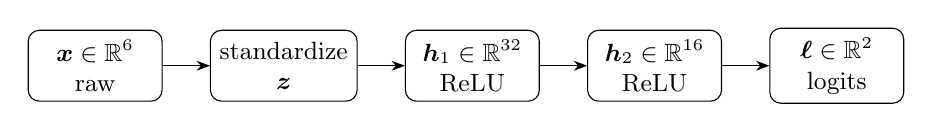
\begin{tikzpicture}[
  box/.style={draw, rounded corners, minimum height=0.9cm, minimum width=1.7cm, align=center, font=\small},
  >={Stealth}]
  \node[box] (x) {$\bm{x}\in\R^6$\\raw};
  \node[box, right=0.6cm of x] (z) {standardize\\$\bm{z}$};
  \node[box, right=0.6cm of z] (h1) {$\bm{h}_1\in\R^{32}$\\ReLU};
  \node[box, right=0.6cm of h1] (h2) {$\bm{h}_2\in\R^{16}$\\ReLU};
  \node[box, right=0.6cm of h2] (o) {$\bm{\ell}\in\R^2$\\logits};
  \draw[->] (x) -- (z); \draw[->] (z) -- (h1); \draw[->] (h1) -- (h2); \draw[->] (h2) -- (o);
\end{tikzpicture}
\caption{The exported graph takes raw values and returns logits, with
standardization inside. The ONNX file contains three \code{Gemm} and two
\code{Relu} operators.}
\label{fig:arch}
\end{figure}

The network is a fully connected MLP (\cref{fig:arch}):
\begin{align}
  \bm{h}_1 &= \relu(\bm{W}_1 \bm{z} + \bm{b}_1), & \bm{W}_1 &\in \R^{32\times 6}, \\
  \bm{h}_2 &= \relu(\bm{W}_2 \bm{h}_1 + \bm{b}_2), & \bm{W}_2 &\in \R^{16\times 32}, \\
  \bm{\ell} &= \bm{W}_3 \bm{h}_2 + \bm{b}_3, & \bm{W}_3 &\in \R^{2\times 16}, \\
  f_{\bm\theta}(\bm{x})_c &= \softmax(\bm{\ell})_c = \frac{e^{\ell_c}}{\sum_{c'} e^{\ell_{c'}}},
\end{align}
with $\relu(u) = \max(0, u)$ applied elementwise. The parameter count is
\begin{equation}
  |\bm\theta| = (6\cdot 32 + 32) + (32\cdot 16 + 16) + (16 \cdot 2 + 2) = 224 + 528 + 34 = 786.
\end{equation}
With two classes the softmax reduces to a logistic function of the logit
difference,
\begin{equation}\label{eq:logistic}
  \hat{p} = \sigma(\ell_1 - \ell_0), \qquad \sigma(u) = \frac{1}{1+e^{-u}},
\end{equation}
so the model is a logistic regression on $16$ learned features.

\section{Training}\label{sec:training}

\subsection{Objective}

The model minimizes the mean, optionally class-weighted, cross-entropy over a
mini-batch $\mathcal{B}$:
\begin{equation}
  \mathcal{L}(\bm\theta) = -\frac{\sum_{i\in\mathcal{B}} w_{y_i} \log f_{\bm\theta}(\bm{x}_i)_{y_i}}{\sum_{i\in\mathcal{B}} w_{y_i}}.
\end{equation}
With \code{class\_weights = "balanced"}, Axon uses inverse-frequency weights over
the $K$ classes of the training labels,
\begin{equation}\label{eq:weights}
  w_c = \frac{N_{\text{tr}}}{K \, N_c},
\end{equation}
which give each class the same total weight. This run used \code{"auto"}, which
applies \cref{eq:weights} only when the largest class is at least three times
the smallest. The full dataset's ratio is $2.57$, so the run very likely trained
with $w_c = 1$; the training-split counts that decide it are not recorded in the
run files.

\subsection{Optimizer}

Parameters are updated with Adam \cite{kingma2015}. With gradient
$\bm{g}_t = \nabla_{\bm\theta}\mathcal{L}$ at step $t$,
\begin{align}
  \bm{m}_t &= \beta_1 \bm{m}_{t-1} + (1-\beta_1)\bm{g}_t, &
  \bm{v}_t &= \beta_2 \bm{v}_{t-1} + (1-\beta_2)\bm{g}_t^{\odot 2}, \\
  \hat{\bm{m}}_t &= \frac{\bm{m}_t}{1-\beta_1^t}, &
  \hat{\bm{v}}_t &= \frac{\bm{v}_t}{1-\beta_2^t}, \\
  \bm\theta_t &= \bm\theta_{t-1} - \eta \, \frac{\hat{\bm{m}}_t}{\sqrt{\hat{\bm{v}}_t} + \epsilon},
\end{align}
with learning rate $\eta = 10^{-3}$ and the burn library's defaults
$\beta_1 = 0.9$, $\beta_2 = 0.999$ and $\epsilon = 10^{-5}$. The batch size is
$32$, so one epoch is $640/32 = 20$ steps and $20$ epochs give $400$ steps. The
training rows are reshuffled each epoch with a permutation seeded by the run
seed and the epoch, so a run is reproducible.

\subsection{Checkpoint selection}

After each epoch $e$ the validation loss $\mathcal{L}_{\text{val}}^{(e)}$ is
computed, and the checkpoint kept is
\begin{equation}
  e^\star = \arg\min_{e \in \{1,\dots,20\}} \mathcal{L}_{\text{val}}^{(e)} = 18,
  \qquad \mathcal{L}_{\text{val}}^{(18)} = 0.3341.
\end{equation}

\section{Results}\label{sec:results}

\begin{figure}[htbp]
\centering
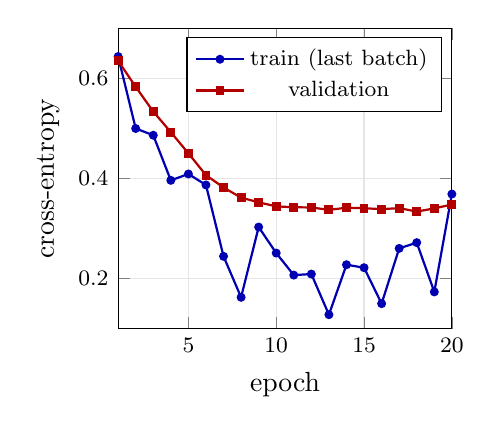
\begin{tikzpicture}
\begin{axis}[
  width=0.48\textwidth, height=5.4cm,
  xlabel={epoch}, ylabel={cross-entropy},
  xmin=1, xmax=20, ymin=0.1, ymax=0.7,
  legend style={font=\footnotesize, at={(0.97,0.97)}, anchor=north east},
  grid=major, grid style={gray!20}, tick label style={font=\footnotesize}]
\addplot[thick, blue!70!black, mark=*, mark size=1.2pt] coordinates {
(1,0.6435)(2,0.4999)(3,0.4864)(4,0.3964)(5,0.4091)(6,0.3872)(7,0.2448)(8,0.1630)(9,0.3032)(10,0.2513)
(11,0.2073)(12,0.2094)(13,0.1283)(14,0.2280)(15,0.2221)(16,0.1504)(17,0.2606)(18,0.2721)(19,0.1738)(20,0.3690)};
\addlegendentry{train (last batch)}
\addplot[thick, red!70!black, mark=square*, mark size=1.2pt] coordinates {
(1,0.6353)(2,0.5829)(3,0.5337)(4,0.4926)(5,0.4503)(6,0.4069)(7,0.3820)(8,0.3620)(9,0.3525)(10,0.3445)
(11,0.3427)(12,0.3423)(13,0.3375)(14,0.3418)(15,0.3408)(16,0.3389)(17,0.3410)(18,0.3341)(19,0.3404)(20,0.3482)};
\addlegendentry{validation}
\end{axis}
\end{tikzpicture}\hfill
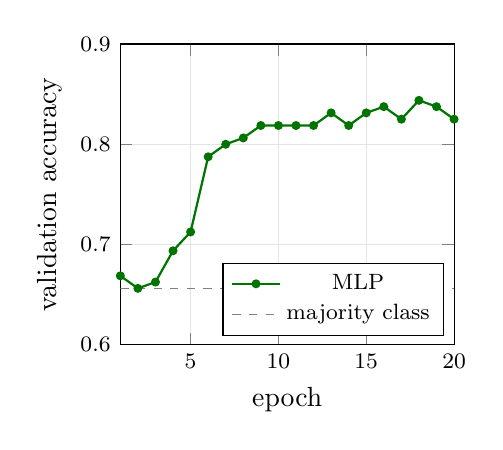
\begin{tikzpicture}
\begin{axis}[
  width=0.48\textwidth, height=5.4cm,
  xlabel={epoch}, ylabel={validation accuracy},
  xmin=1, xmax=20, ymin=0.6, ymax=0.9,
  grid=major, grid style={gray!20}, tick label style={font=\footnotesize},
  legend style={font=\footnotesize, at={(0.97,0.03)}, anchor=south east}]
\addplot[thick, green!45!black, mark=*, mark size=1.2pt] coordinates {
(1,0.6687)(2,0.6562)(3,0.6625)(4,0.6937)(5,0.7125)(6,0.7875)(7,0.8000)(8,0.8063)(9,0.8187)(10,0.8187)
(11,0.8187)(12,0.8187)(13,0.8313)(14,0.8187)(15,0.8313)(16,0.8375)(17,0.8250)(18,0.8438)(19,0.8375)(20,0.8250)};
\addlegendentry{MLP}
\addplot[dashed, gray] coordinates {(1,0.65625)(20,0.65625)};
\addlegendentry{majority class}
\end{axis}
\end{tikzpicture}
\caption{Validation loss flattens after epoch $10$ and is lowest at epoch $18$,
where accuracy also peaks. The training curve is the loss of each epoch's last
mini-batch, which is why it is noisy.}
\label{fig:curves}
\end{figure}

\subsection{Metrics}

From the confusion matrix with true positives $TP$, false positives $FP$,
false negatives $FN$ and true negatives $TN$, taking churn as the positive class:
\begin{gather}
  \text{Acc} = \frac{TP + TN}{TP+FP+FN+TN}, \quad
  P = \frac{TP}{TP + FP}, \quad
  R = \frac{TP}{TP + FN}, \\
  \text{Spec} = \frac{TN}{TN + FP}, \quad
  F_1 = \frac{2PR}{P + R}.
\end{gather}
Because $n = 160$ is small, we report a Wilson score interval
\cite{wilson1927} for accuracy, at $z = 1.96$:
\begin{equation}
  \frac{\hat{p} + \frac{z^2}{2n}}{1 + \frac{z^2}{n}} \pm
  \frac{z}{1 + \frac{z^2}{n}}\sqrt{\frac{\hat{p}(1-\hat{p})}{n} + \frac{z^2}{4n^2}}.
\end{equation}

\begin{table}[htbp]
\centering
\caption{Validation confusion matrices (rows: true class; columns: predicted).
The two checkpoints differ only in three churners missed at epoch $20$.}
\label{tab:cm}
\begin{tabular}{l cc @{\hspace{2.5em}} cc}
\toprule
 & \multicolumn{2}{c}{Epoch 18 (kept)} & \multicolumn{2}{c}{Epoch 20 (last)} \\
\cmidrule(lr){2-3}\cmidrule(lr){4-5}
 & pred.\ stayed & pred.\ churned & pred.\ stayed & pred.\ churned \\
\midrule
stayed  & 95 & 10 & 95 & 10 \\
churned & 15 & 40 & 18 & 37 \\
\bottomrule
\end{tabular}
\end{table}

\begin{table}[htbp]
\centering
\caption{Validation metrics ($n = 160$). The kept checkpoint beats the
majority-class baseline by about $19$ points of accuracy, and the baseline's
interval does not overlap it.}
\label{tab:metrics}
\begin{tabular}{l S[table-format=1.3] S[table-format=1.3] S[table-format=1.3]}
\toprule
Metric & {Epoch 18} & {Epoch 20} & {Baseline} \\
\midrule
Accuracy          & 0.844 & 0.825 & 0.656 \\
\quad 95\% Wilson interval & {[0.780, 0.892]} & {[0.759, 0.876]} & {[0.580, 0.725]} \\
Precision (churn) & 0.800 & 0.787 & {n/a} \\
Recall (churn)    & 0.727 & 0.673 & 0.000 \\
Specificity       & 0.905 & 0.905 & 1.000 \\
$F_1$ (churn)     & 0.762 & 0.725 & 0.000 \\
\bottomrule
\end{tabular}
\end{table}

The kept checkpoint finds $40$ of the $55$ churners while flagging $10$ of the
$105$ customers who stayed (\cref{tab:cm,tab:metrics}). Between epochs $18$ and
$20$ the only change is three churners lost to false negatives, the
sensitivity one expects from a validation set this small: one record moves
accuracy by $1/160 = 0.625$ percentage points.

\section{Deployment}\label{sec:deploy}

The model ships as \code{model.onnx} with a sidecar \code{model.json} that
describes the input slots and output classes. The input tensor \code{input}
takes the six raw values in the order of \cref{tab:features}; the output
\code{output} holds the logits for classes $0$ and $1$, and a caller obtains the
churn probability from \cref{eq:logistic}. Because standardization lives in the
graph, the training statistics cannot drift apart from the weights.

\section{Limitations and further work}\label{sec:limits}

\begin{description}
  \item[Synthetic data] The records are generated, so the metrics describe how
        well the MLP recovers the generator's rule, not customer behaviour.
  \item[Small validation set] The accuracy interval spans about eleven points;
        $k$-fold cross-validation would give a steadier estimate.
  \item[Threshold and calibration] The decision threshold is $0.5$. When a
        missed churner costs $c_{FN}$ and a wasted retention offer costs
        $c_{FP}$, the cost-minimizing threshold for a calibrated $\hat{p}$ is
        $\tau^\star = c_{FP}/(c_{FP} + c_{FN})$. Calibration has not been
        checked; a reliability diagram or the Brier score
        $\frac{1}{n}\sum_i (\hat{p}_i - y_i)^2$ would come first.
  \item[Baselines] Only the majority-class baseline was run. A logistic
        regression on $\bm{z}$ and a gradient-boosted tree model would show
        how much the hidden layers add.
\end{description}

\section*{Preparation}

This report was drafted with an AI assistant (Claude) from the project's files
and checked against them; the author is responsible for its content. Every
number is traced to its source in \cref{app:provenance}.

\begin{thebibliography}{9}
\bibitem{kingma2015} D.~P. Kingma and J.~Ba. Adam: A method for stochastic
  optimization. In \emph{International Conference on Learning Representations}, 2015.
\bibitem{wilson1927} E.~B. Wilson. Probable inference, the law of succession,
  and statistical inference. \emph{Journal of the American Statistical
  Association}, 22(158):209--212, 1927.
\end{thebibliography}

\appendix
\section{Provenance of numbers}\label{app:provenance}

\begin{table}[htbp]
\centering
\caption{Where each reported number comes from. Paths are relative to the
project folder, and \code{RUN} stands for the training run's folder, given
below the table.}
\label{tab:provenance}
\small
\begin{tabular}{>{\raggedright\arraybackslash}p{0.42\textwidth} >{\raggedright\arraybackslash}p{0.52\textwidth}}
\toprule
Number & Source \\
\midrule
$N = 800$, feature statistics, class counts, churn by contract & computed from \code{data/customers.csv} \\
Split sizes, seed, batch size, learning rate, epochs, \code{"auto"} weights & \code{train.toml}, \code{RUN/config.json}, \code{RUN/metrics.jsonl} (log line) \\
Training-split $\mu_j$, $\sigma_j$ & \code{model.json}, \code{RUN/checkpoints/best.json} \\
Loss and accuracy per epoch, best epoch & \code{RUN/metrics.jsonl}, \code{RUN/summary.json} \\
Confusion matrices & \code{RUN/artifacts/cm-epoch18.json}, \code{cm-epoch20.json} \\
Graph operators & \code{model.onnx} (operator names) \\
Class-weight rule, ReLU, seeded shuffle & Axon v0.9.0 source (\code{tabular.rs}, \code{model.rs}); installed \code{axon} is v0.9.0 \\
Adam $\beta_1, \beta_2, \epsilon$ & \code{burn-optim} 0.21.0, \code{AdamConfig} defaults \\
Derived: parameter count, precision, recall, $F_1$, Wilson intervals, baseline & computed from the rows above \\
\bottomrule
\end{tabular}
\end{table}

The project folder is \code{synapse-demo/churn-risk}, and the run folder
inside it is
\[
  \code{.nexis-ml/runs/2026-11-27-0343-tabular}.
\]

\paragraph{Not confirmed.} The run files do not record which Axon binary Nexis
invoked or the training split's class counts, so whether class weighting
switched on is inferred, not observed.

\end{document}
